\documentclass{beamer}
\mode<presentation>
{
	\usetheme{Szeged}
%	\usecolortheme{beaver}
}
\title{TJ-II}
\author{K.A. Blondino and C.J. Col\'{o}n}
\institute[TU/e]{Eindhoven University of Technology}


\usepackage{amsmath, graphicx}
\usepackage{natbib, framed}

\usepackage[orientation=portrait,size=a0,scale=1.4,debug]{beamerposter}
\usetheme{confposter}

% SET UP SOME LENGTHS
\newlength{\sepwidsingle}
\newlength{\sepwiddouble}
\newlength{\onecolwid}
\setlength{\sepwidsingle}{0.005\paperwidth} % Separation width (white space) between columns
\setlength{\sepwiddouble}{0.01\paperwidth}
\setlength{\onecolwid}{0.46\paperwidth} % Width of one column

\begin{document}

% All encompassing frame
\begin{frame}[t]

% Initiate the columns
\begin{columns}[t]

% ------------------------------------------
% TU/e LOGOS
\begin{tikzpicture}[remember picture,overlay]
	\node [shift={(8 cm, -4.5 cm)}] at (current page.north west) {
\includegraphics[height=6cm]{../Graphics/tue_fusion_logo.png}};
\end{tikzpicture}

\begin{tikzpicture}[remember picture,overlay]
	\node [shift={(-15 cm, -4.5 cm)}] at (current page.north east) {
\includegraphics[height=5.5cm]{../Graphics/tuelogo.pdf}};
\end{tikzpicture}

% DEVICE SCHEMATIC
\begin{tikzpicture}[remember picture,overlay]
	\node [shift={(22.5 cm, -4.5 cm)}] at (current page.north west) {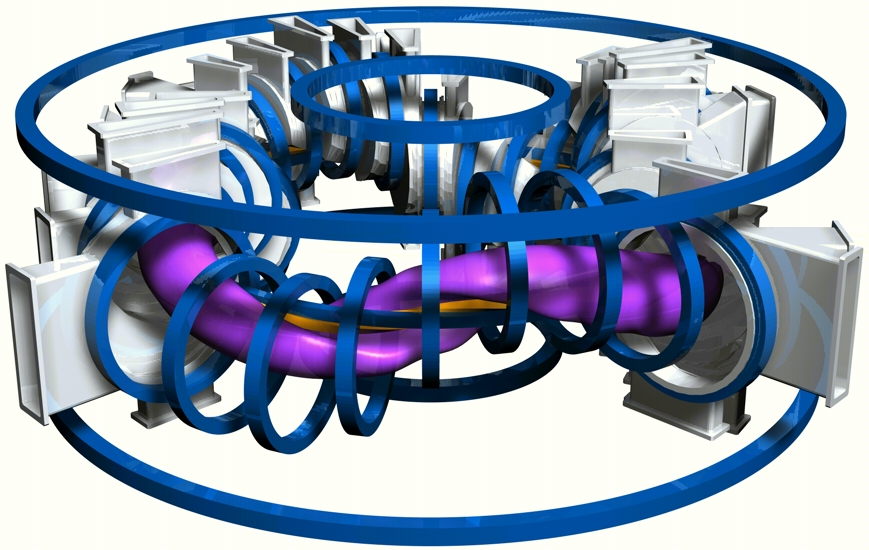
\includegraphics[height=7.5cm]{../Graphics/TJII_model.jpg}};
\end{tikzpicture}
% ------------------------------------------

%\begin{column}{\sepwiddouble}\end{column}

%-----------------------------------------------------------

% Left-hand side column
\begin{column}{\onecolwid}

\begin{alertblock}{Basic Specifications}
\begin{itemize}
	\item Located in the National Fusion Laboratory of Spain; first plasma in 1997
	\item Discharges last $\approx\,25$ ms \cite{tj-ii_nodate}
	\item Magnetic flexibility, \emph{i.e.} rotational transform can be widely varied \cite{ascasibar_overview_2001}
	\item Periodicity of 4
	\item Low Magnetic Shear, \emph{i.e.} flat $\iota$-profile \cite{alejaldre_first_1999}
	\item Modular vacuum vessel with 96 ports \cite{tj-ii_nodate}
	\item $\langle R \rangle \,=\, 1.5$ m, $\langle a \rangle \,=\, 0.22$ m, $B \,=\, 1.2$ T
	\item Heating: ECRH of 600 kW and NBI of 3 MW \cite{ascasibar_overview_2001}
	\item First plasmas achieved $n \,=\, 1.2\times 10^{19}$ m$^{-3}$ and $T_e \,=\, 2$ keV \cite{alejaldre_first_1999}
\end{itemize}
\end{alertblock}

\begin{block}{Magnetic Configuration}

\hspace{32pt} The device consists of 32 toroidal-field water-cooled copper coils, one helical coil ($I_\text{max} = 260$ kA), made of two subcoils individually supplied to control shear, and one circular coil ($I_\text{max} = 280$ kA). Together, they produce the ``bean''-shaped flux surfaces.

%\begin{framed}
\begin{figure}
	\resizebox{1.0\textwidth}{!}
	{
		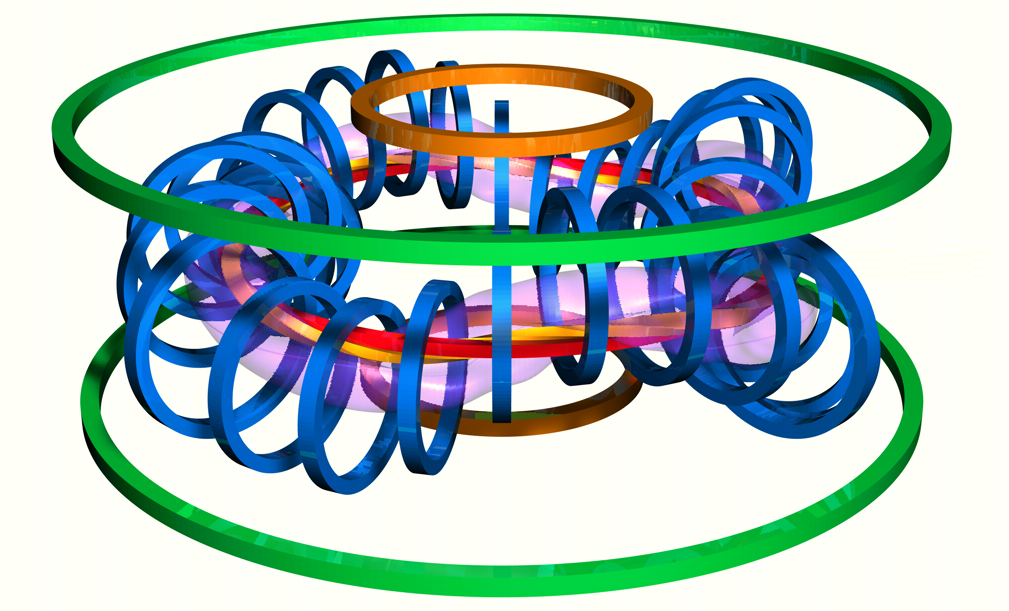
\includegraphics[height=20cm]{../Graphics/TJ-II_Coils.png}
		\quad
		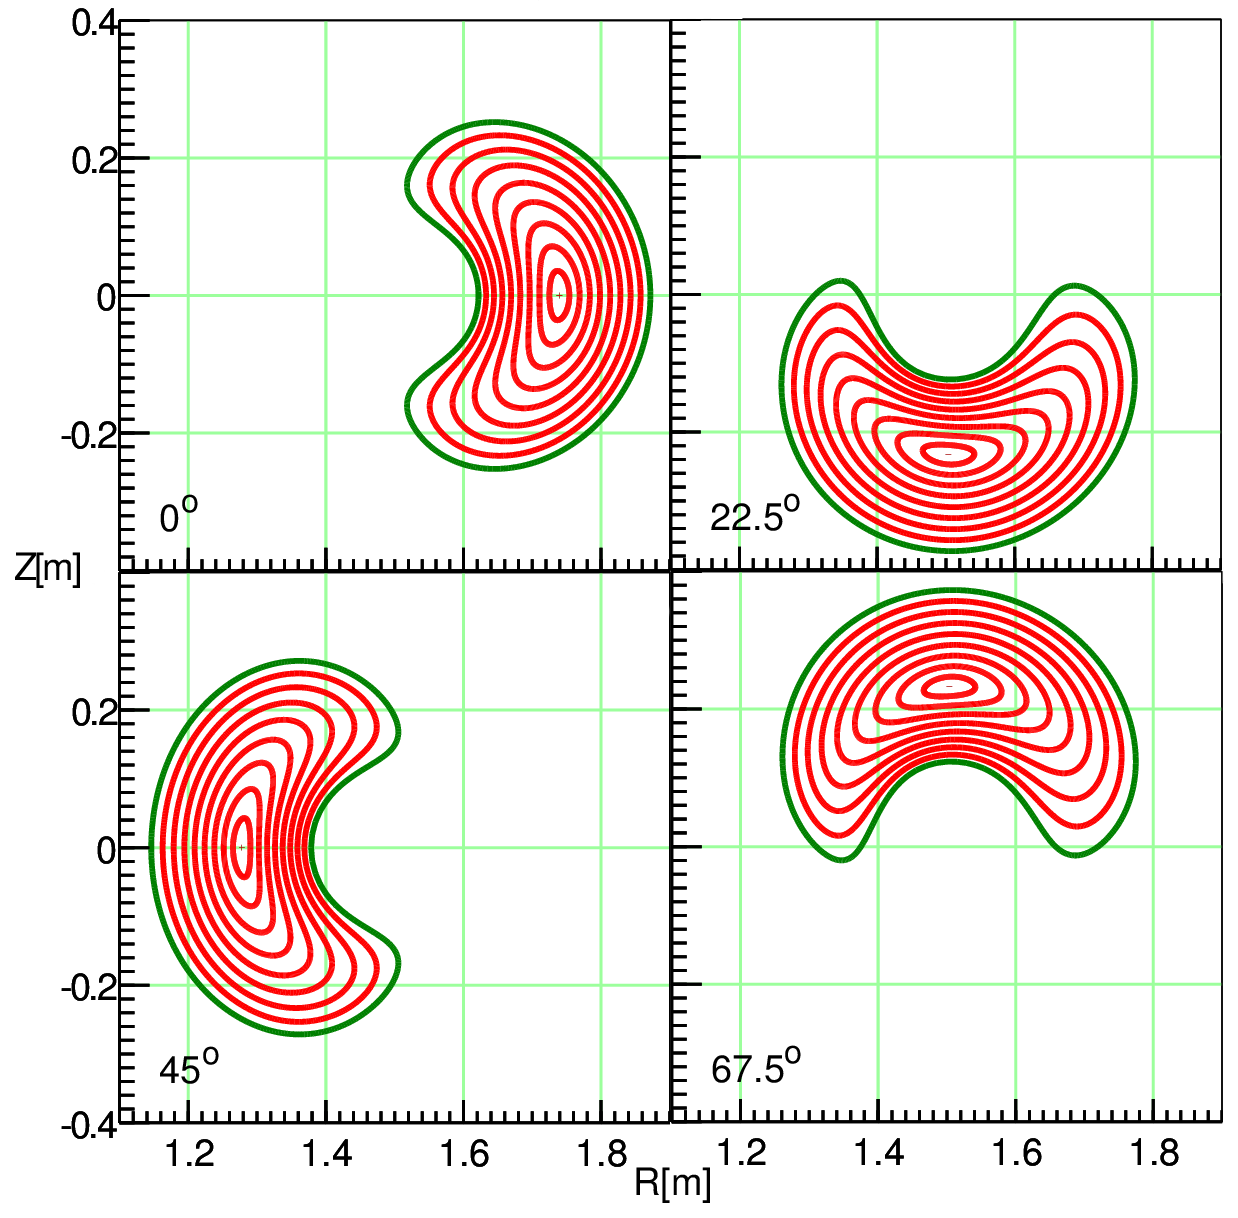
\includegraphics[height=20cm]{../Graphics/flux_surfaces.png}
	}
	\caption{\textbf{LEFT:} Color-labeled coils. Red: central, yellow: helical, blue: toroidal, green: vertical, brown: radial. \textbf{RIGHT:} Magnetic flux surfaces at different toroidal angles.}
	\label{fig:magnetic_coils}
\end{figure}
%\end{framed}
\vspace{-0.2cm}
\begin{equation*}
	B \,=\, B_0 \sum_{m,n} a_{m,n}\left(\psi\right) \cos\left(m\theta - n\phi\right)
\end{equation*}

\hspace{32pt} The magnetic field can be represented as a Fourier series in Boozer coordinates, shown in the above equation. The three main harmonics of the field (toroidicity, helicity, and corner ripple) produce the magnetic topology shown in Fig.~\ref{fig:magnetic_field} \cite{solano_study_1988}.

\begin{figure}
	\resizebox{1.0\textwidth}{!}
	{
		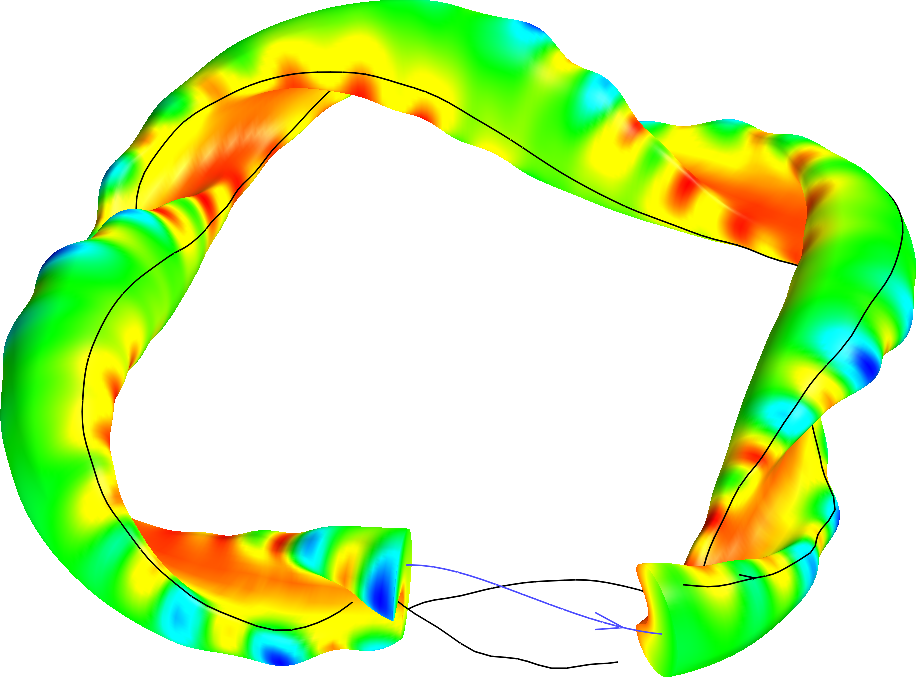
\includegraphics[trim={0 0 0 -0.5cm},clip,height=20cm]{../Graphics/magnetic_field_2.png}
		\quad
		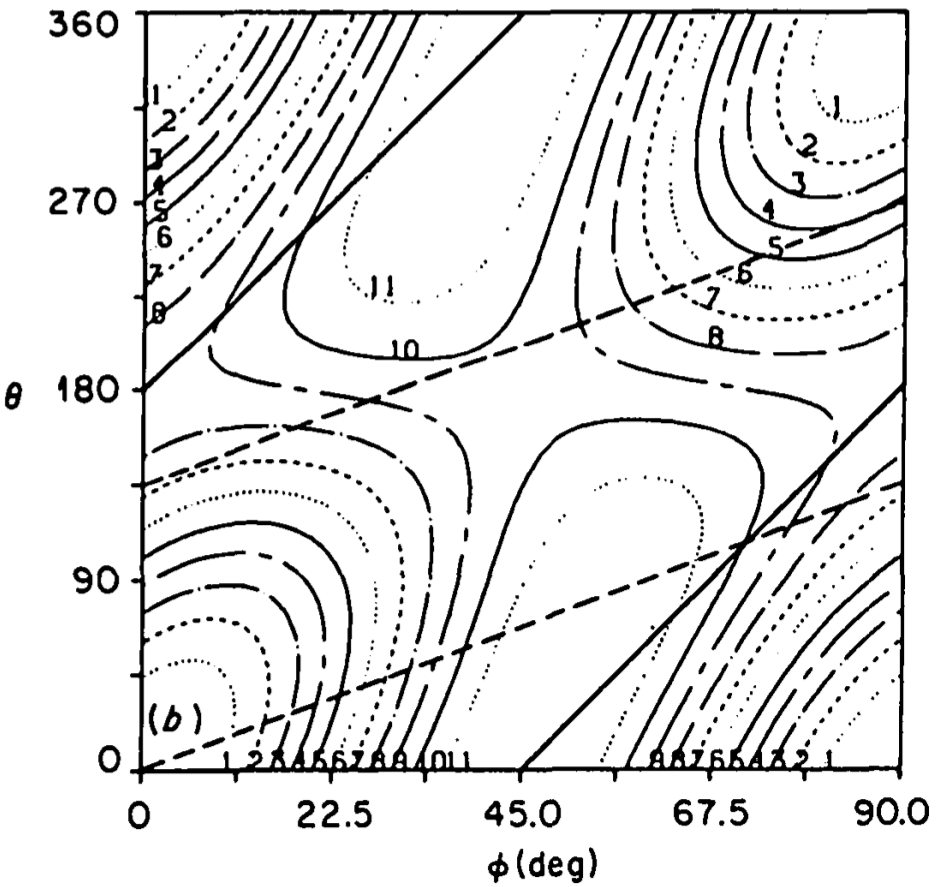
\includegraphics[height=20cm]{../Graphics/Bcontours.png}
	}
	\caption{\textbf{LEFT:} Magnetic field strength on the outermost flux surface. Red corresponds to high field magnitude and blue corresponds to low magnitude. \textbf{RIGHT:} Magnetic topology produced using the three main harmonics.}
	\label{fig:magnetic_field}
\end{figure}

\end{block}

\begin{block}{Neoclassical Transport}

\hspace{32pt} In Fig.~\ref{fig:drifts}, the particle radial drifts present in TJ-II and how they are mitigated by a radial electric field are illustrated \cite{solano_study_1988}.

\begin{figure}
	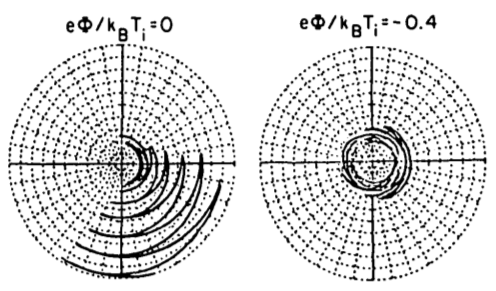
\includegraphics[width=0.7\linewidth]{../Graphics/Drifts.png}
	\caption{The drifts of particles with and without a radial electric field.}
	\label{fig:drifts}
\end{figure}

\end{block}

\end{column}

%-----------------------------------------------------------

% Tiny separating column of white space
\begin{column}{\sepwidsingle}\end{column}
\vrule
\begin{column}{\sepwidsingle}\end{column}

%-----------------------------------------------------------

% Right-hand side column
\begin{column}{\onecolwid}

\begin{figure}
	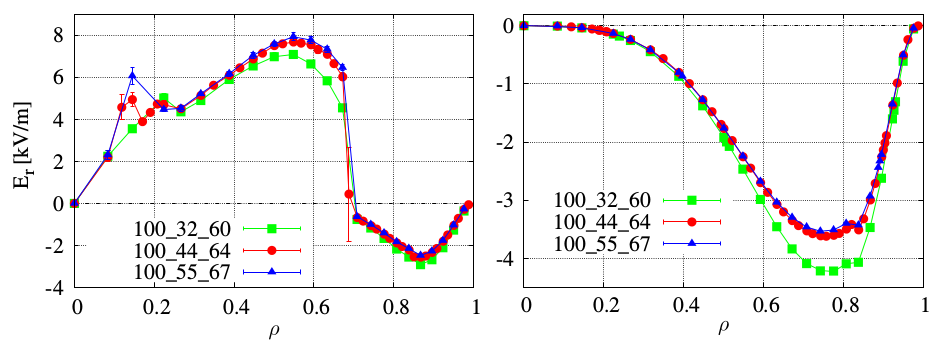
\includegraphics[trim={0 0.5cm 0 0.5cm}, clip, width=1.0\linewidth]{../Graphics/Radial_field.png}
	\caption{Calculations of the ambipolar radial electric field versus normalized minor radius. The left has a low, flat density profile and the right has a higher pedestal-like density profile. These results are in qualitative agreement with experiment \cite{velasco_study_2012}.}
	\label{fig:radial_field}
\end{figure}

\textrm{\hspace{32pt} The appearance of the radial electric field due the disparity between particle fluxes has been confirmed \cite{velasco_study_2012}. The sign of the field depends on the density; a low-density ECRH plasma has mostly-positive sign while a high-density NBI plasma is negative, shown in Fig.~\ref{fig:radial_field}. \\ \hspace{32pt} Calculations result in a \emph{textbook} diffusion coefficient as illustrated by Fig.~\ref{fig:diffusion}. In the low-collisionality regime, the radial electric field suppresses neoclassical transport.}

\begin{figure}
	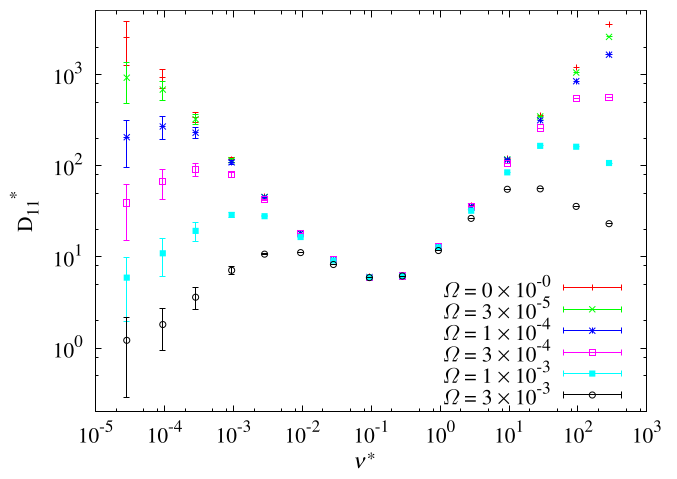
\includegraphics[trim={0 0.4cm 0 0.2cm},clip, width=0.7\linewidth]{../Graphics/Diffusion.png}
	\caption{Calculated diffusion coefficient as a function of collisionality, over a scan of $\Omega$, the normalized radial electric field \cite{velasco_study_2012}.}
	\label{fig:diffusion}
\end{figure}

\begin{block}{Shortcomings}
\begin{itemize}
	\item The device has no form of quasi-symmetry.
	\item It has an estimated bootstrap current density of $1.4$ A/cm$^2$, inferred by the unexpected rotational velocities from ions. This limits the achievable $\beta$ \cite{rapisarda_investigation_2005}.
	\item ELM-like events have been observed at plasma energies above 1 kJ \cite{ascasibar_overview_2001}.
	\item At first plasmas He impurities were accumulated, this was mostly solved by Li coating. Together with vacuum vessel groove acting as a limiter, this causes radiative collapse, limiting the achievable density \cite{sanchez_confinement_2009}.
\end{itemize}
\end{block}

\begin{block}{Possible Improvement}

\begin{figure}
	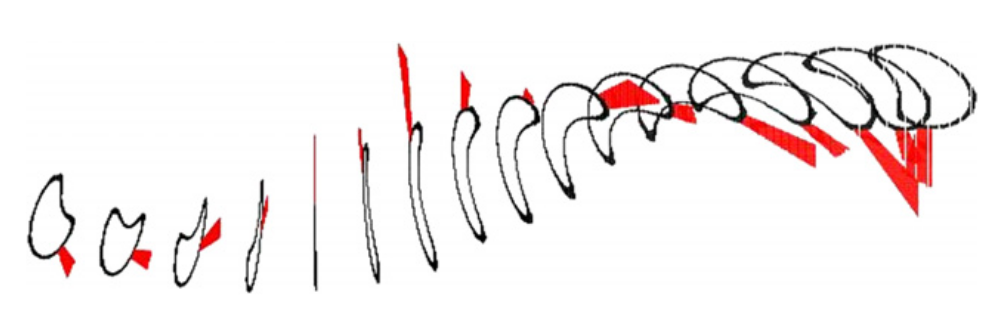
\includegraphics[trim={0 1.1cm 0 1.7cm}, clip, width=0.6\linewidth]{../Graphics/Divertor.png}
	\caption{Proposed flux-expansion divertor locations \cite{castejon_flux-expansion_2009}.}
\end{figure}

\begin{itemize}
	\item To reduce the high amount of magnetic ripple, either introduce additional coils or improving existing ones (see Fig.~\ref{fig:magnetic_field}).
	\item The inclusion of a flux-expansion divertor is an improvement considered for the machine \cite{castejon_flux-expansion_2009}. This requires the existence of ergodic zones, which are possible to create with additional perturbative coils. This would increase the achievable confinement time.
\end{itemize}

\end{block}

\begin{block}{References}
	\setbeamertemplate{bibliography item}[text]
	\bibliographystyle{plain}
%	\nocite{*}
	\begin{scriptsize}
		\bibliography{../References/References}
	\end{scriptsize}
\end{block}


\end{column}

\begin{column}{\sepwiddouble}\end{column}

\end{columns}

\end{frame}
\end{document}